\documentclass[10pt]{beamer}

\usetheme{CambridgeUS}
\usepackage[english, russian]{babel}
\usepackage[utf8]{inputenc}
\usepackage{caption}
\usepackage{etoolbox}
\usepackage{multicol}
\usepackage{listings}
\usepackage{color}

\definecolor{mygreen}{rgb}{0,0.6,0}
\lstset{
  basicstyle=\ttfamily\footnotesize,        % the size of the fonts that are used for the code
  breaklines=true,                 % automatic line breaking only at whitespace
  captionpos=b,                    % sets the caption-position to bottom
  commentstyle=\color{mygreen},    % comment style
  keywordstyle=\color{blue},       % keyword style
  stringstyle=\color{red},     % string literal style
  showstringspaces=false,
  morekeywords={include, printf},
  texcl=true     %<---- added
}

\title[\href{https://goo.gl/NRgp8K}{https://goo.gl/NRgp8K} (Term 1)]{Компиляция и линковка}
\author[Гусев Илья, Булгаков Илья]{Гусев Илья, Булгаков Илья}
\institute[МФТИ] 
{Московский физико-технический институт\\*}
\date{Москва, 2018}
\subject{Computer Science}

\begin{document}

\begin{frame}
  \titlepage
\end{frame}

\begin{frame}{Содержание}
\tableofcontents
\end{frame}

\section{После исходного кода}
\subsection{Общая схема}
\begin{frame}[fragile]{Общая схема}

\begin{multicols}{2}
g++ prog1.cpp
\begin{enumerate}
\item Препроцессор копирует содержимое включённых файлов в исходный код, разворачивает макросы и подставляет константы, переопределённые с помощью \#define.
\item Развёрнутый исходный код компилируется в платформозависимый ассемблер (.s). Включение вывода: \-\-save\-temps
\item Ассемблерный код собирается в объектный код платформы (.o). Смотреть: nm, objdump.
\item Объектный код связывается с другими объектными файлами и библиотеками.
\end{enumerate}
\vfill\eject
 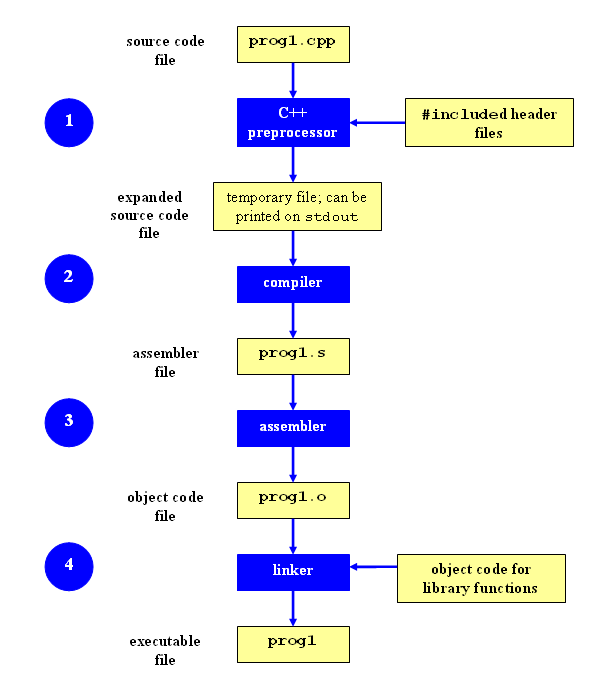
\includegraphics[width=6cm, height=6.5cm]{Term_3/Source/Pictures/compile.png}
\end{multicols}
\end{frame}

\subsection{Компиляция}
\begin{frame}[fragile]{Компиляция}
\begin{enumerate}
    \item Токенизация
    \item Построение промежуточного дерева по грамматике
    \item Построение abstract-syntax tree (AST)
    \item Построение платформо-зависимого дерева
    \item Создание ассемблерного кода.
\end{enumerate}
\end{frame}

\subsection{Линковка}
\begin{frame}[fragile]{Линковка}
На выходе с компилятора приходят объектные файлы. Они ничего не знают о существовании друг друга и их надо объединить в один, заполнив их "пропуски". Пример одиночного объектного файла:
 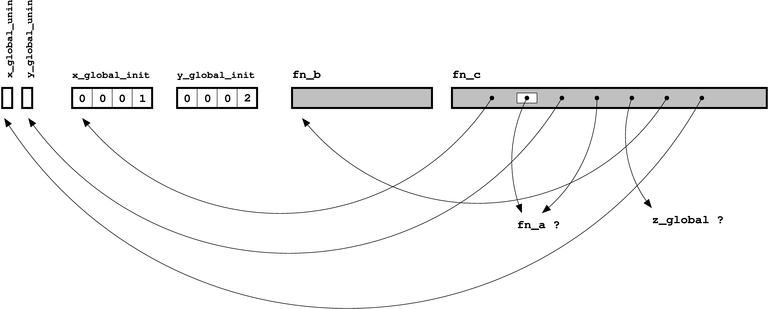
\includegraphics[width=12cm, height=5cm]{Term_3/Source/Pictures/c_parts.png}
\end{frame}

\begin{frame}[fragile]{Линковка - собранный файл}
Пример собранного исполняемого файла:
 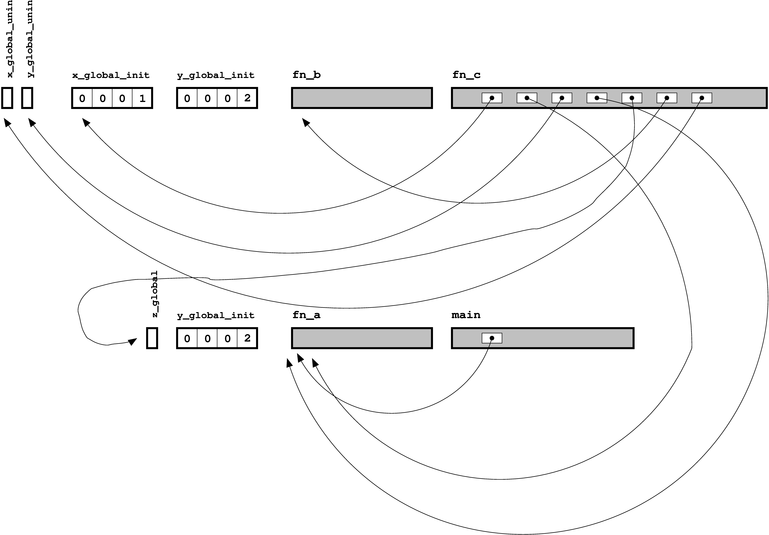
\includegraphics[width=10cm, height=7cm]{Term_3/Source/Pictures/c_parts_linked.png}
\end{frame}

\subsection{Загрузка исполняемого файла}
\begin{frame}{Загрузка исполняемого файла}
\begin{enumerate}
\item Глобальные переменные кладутся в память процесса as is.
\item Локальные переменные кладутся на стек, который растёт при вызовах функций и уменьшается при их завершении.
\item Динамические переменные расходуют память кучи, системные malloc и free управляют этой частью процесса.
\item bss - фрагмент неинициализированных пременных, заполнен нулями
\item Кроме того, на затронут mapping файлов в память и пространство ядра (kernel space).
\end{enumerate}
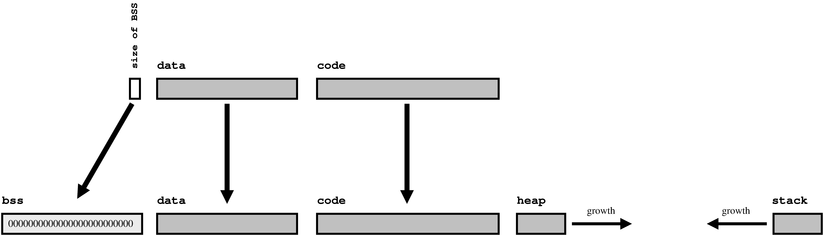
\includegraphics[width=11cm, height=3cm]{Term_3/Source/Pictures/os_map.png}
\end{frame}

\section{Библиотеки}
\subsection{Статические библиотеки}
\begin{frame}{Статические библиотеки}
\begin{enumerate}
\item Самая простая версия библиотек
\item Linux: lib*.a, Windows: *.lib
\item Библиотека может состоять из нескольких .o файлов.
\item Библиотека участвует в линковке объектными файлами, то есть тянется не вся библиотека, а только объектники, которые заполняют какой-либо 'пропуск'. При этом, тянется всё, что есть в этом объектном файле, в том числе новые 'пропуски'.
\item Линковка библиотек только после линковки частей программы, и только если есть 'пропуски'.
\item Библиотеки линкуются строго по порядку. Если вдруг библиотека-2 (идущая после библиотеки-1) требует что-то, что есть в незагруженном объектнике библиотеки-1, линкер это что-то не найдёт!

\end{enumerate}
\end{frame}

\subsection{Shared библиотеки}
\begin{frame}{Проблемы статических библиотек}
\begin{enumerate}
\item Каждый исполняемый файл содержит копию библиотеки $\rightarrow$ исполняемые файлы занимают кучу места.
\item Если мы хотим поменять код библиотеки нужно перелинковывать ВСЕ исполняемые файлы.
\end{enumerate}
\end{frame}

\subsection{Shared библиотеки}
\begin{frame}{Shared библиотеки}
\begin{enumerate}
\item *.so, *.dll, *.dylib.
\item Линкер просто оставляет некоторые 'пропуски' открытыми, записывая, что они должны заполняться из такой-то shared библиотеки.
\item Код библиотеки не включается в исполняемый файл.
\item Во время запуска программы (до исполнения main) операционная система натравливает маленькую версию линкера (ld.so) на оставшиеся 'пропуски'.
\item Если мы захотим поменять код, скажем, printf - нам не нужно перелинковывать все исполняемые файлы. 
\item Загрузка shared библиотек происходит целиком, а не по объектным файлам!
\item $ldd$ <имя исполняемого файла> чтобы посмотреть, какие библиотеки он захватывает.
\end{enumerate}
\end{frame}

\subsection{Динамически загружаемые библиотеки}
\begin{frame}{Динамически загружаемые библиотеки (настоящие DLL)}
\begin{enumerate}
\item Загрузка бибилиотеки в любом месте программы, не только до main.
\item dlopen и dlsym (или LoadLibrary и GetProcAddress).
\item dlopen - берёт библиотеку и загружает её в память процесса.
\item dlsym - берёт имя символа и возвращает указатель на его местонахождение в в загруженной области памяти.
\end{enumerate}
\end{frame}

\section{C++ - mangling}
\subsection{Перегрузка функций}
\begin{frame}{Перегрузка функций}
\begin{enumerate}
\item В Си нельзя перегружать функции, в C++ можно.
\item Пример: int max(int x, int y); float max(float x, float y);
\item А что делать линкеру, он же по имени символы ищет?
\end{enumerate}
\end{frame}

\begin{frame}{Mangling}
\begin{enumerate}
\item Решение: {
\begin{enumerate}
    \item int max(int x, int y) -> имя - \_Z3maxii
    \item float max(float x, float y) -> имя - \_Z3maxff
\end{enumerate}
}
\item Всё сложнее для классов.
\item И ещё сложнее для шаблонов.
\item extern \quotes{C} у объявления и определения - убирает mangling для совместимости кода на Си и C++.
\item extern \quotes{C} игнорируется методами класса.
\end{enumerate}
\end{frame}

\appendix
\section<presentation>*{\appendixname}
\subsection<presentation>*{Useful links}

\begin{frame}[allowframebreaks]
  \frametitle<presentation>{Полезные ссылки}
    
  \begin{thebibliography}{10}
{
  \beamertemplatebookbibitems
  % Start with overview books.
    
\bibitem{standard}
  \texttt{C++11 n3690}
  \newblock \href{http://www.open-std.org/jtc1/sc22/wg21/docs/papers/2013/n3690.pdf}{\texttt{http://www.open-std.org/jtc1/sc22/wg21/docs/\\papers/2013/n3690.pdf}}

  \bibitem{link01}
  \texttt{Статья про линковку}
  \newblock \href{https://www.lurklurk.org/linkers/linkers.html#cfile}{\texttt{https://www.lurklurk.org/linkers/linkers.html#cfile}}
  
    \bibitem{compilation-schema}
  \texttt{The C++ compilation process}
   \newblock \href{http://faculty.cs.niu.edu/~mcmahon/CS241/Notes/compile.html}{\texttt{ http://faculty.cs.niu.edu/~mcmahon/CS241/Notes/compile.html}}
   
    \bibitem{memory}
  \texttt{Хабр: Организация памяти}
   \newblock \href{https://habrahabr.ru/company/smart_soft/blog/185226/}{\texttt{https://habrahabr.ru/company/smart_soft/blog/185226/}}
   
  
}
    
  \end{thebibliography}
\end{frame}

\end{document}


